
%(BEGIN_QUESTION)
% Copyright 2008, Tony R. Kuphaldt, released under the Creative Commons Attribution License (v 1.0)
% This means you may do almost anything with this work of mine, so long as you give me proper credit

Many flammable gases are produced in oil refining processes as ``waste'' products.  These ``waste'' gases may be used as fuel for steam boilers and combustion heaters in other parts of the refinery.  The problem is, ``waste'' fuel gas production is often unsteady, and the demand for fuel gas in boilers and heaters is unsteady as well.  There are times when there will be a surplus of waste gas (more than can be used), and times when there will not be enough.

$$\includegraphics[width=15.5cm]{i01711x01.eps}$$

The above pressure control system works to maintain constant fuel gas pressure in the accumulator vessel.  When fuel demand exceeds waste gas production, the pressure control system adds purchased natural gas into the accumulator to make up the difference.  When waste gas production exceeds fuel demand, the system vents excess waste gas to the flare where it burns off safely.  The two pressure valves are split-ranged to work from the same 4-20 mA controller output signal.

Identify the proper split-ranges for these two valves, assuming a direct-acting pressure transmitter and a reverse-acting controller (in each box you should write a single milliamp value):

% No blank lines allowed between lines of an \halign structure!
% I use comments (%) instead, so that TeX doesn't choke.

$$\vbox{\offinterlineskip
\halign{\strut
\vrule \quad\hfil # \ \hfil & 
\vrule \quad\hfil # \ \hfil & 
\vrule \quad\hfil # \ \hfil \vrule \cr
\noalign{\hrule}
%
% First row
Valve & Input signal (mA) & Input signal (mA) \cr
%
tag \# & for full-shut & for wide-open \cr
%
\noalign{\hrule}
%
% Another row
PV-45a &  &  \cr
%
\noalign{\hrule}
%
% Another row
PV-45b &  &  \cr
%
\noalign{\hrule}
} % End of \halign 
}$$ % End of \vbox

One fine day the instrument air supply to valve PV-45a fails.  Describe the effect on the accumulator's fuel gas pressure during two different process conditions as a result of this valve failure: when fuel gas demand exceeds waste gas supply, and vice-versa.  Assume pressure valve PV-45b continues to work normally:

\begin{itemize}
\item{} Fuel gas demand exceeds waste gas supply; valve failure results in \underbar{\hskip 100pt}
\vskip 5pt 
\item{} Waste gas supply exceeds fuel gas demand; valve failure results in \underbar{\hskip 100pt}
\end{itemize}

\underbar{file i01711}
%(END_QUESTION)





%(BEGIN_ANSWER)

I recommend +1 point for each valve range value (4 points), and 3 points for correctly describing the effect of each gas demand/supply scenario (6 points).

% No blank lines allowed between lines of an \halign structure!
% I use comments (%) instead, so that TeX doesn't choke.

$$\vbox{\offinterlineskip
\halign{\strut
\vrule \quad\hfil # \ \hfil & 
\vrule \quad\hfil # \ \hfil & 
\vrule \quad\hfil # \ \hfil \vrule \cr
\noalign{\hrule}
%
% First row
Valve & Input signal (mA) & Input signal (mA) \cr
%
tag \# & for full-shut & for wide-open \cr
%
\noalign{\hrule}
%
% Another row
PV-45a & {\bf 12 mA} & {\bf 20 mA} \cr
%
\noalign{\hrule}
%
% Another row
PV-45b & {\bf 12 mA} & {\bf 4 mA} \cr
%
\noalign{\hrule}
} % End of \halign 
}$$ % End of \vbox

If fuel gas demand exceeds waste gas supply, the accumulator pressure will {\bf fall} because it cannot supplement the lack of supply with natural gas.

\vskip 10pt

If waste gas supply exceeds fuel gas demand, the system will {\bf operate normally} (pressure maintained at setpoint).

%(END_ANSWER)





%(BEGIN_NOTES)

{\bf This question is intended for exams only and not worksheets!}.

%(END_NOTES)


